\documentclass[tikz]{standalone}
\usepackage{amsmath}
\usepackage{times}
\usepackage{txfonts}

\usetikzlibrary{arrows}
\usetikzlibrary{intersections}
\usetikzlibrary{math}
\usetikzlibrary{positioning}
\usetikzlibrary{arrows.meta}
\usetikzlibrary{shapes.misc}
\usetikzlibrary{calc}

\begin{document}
  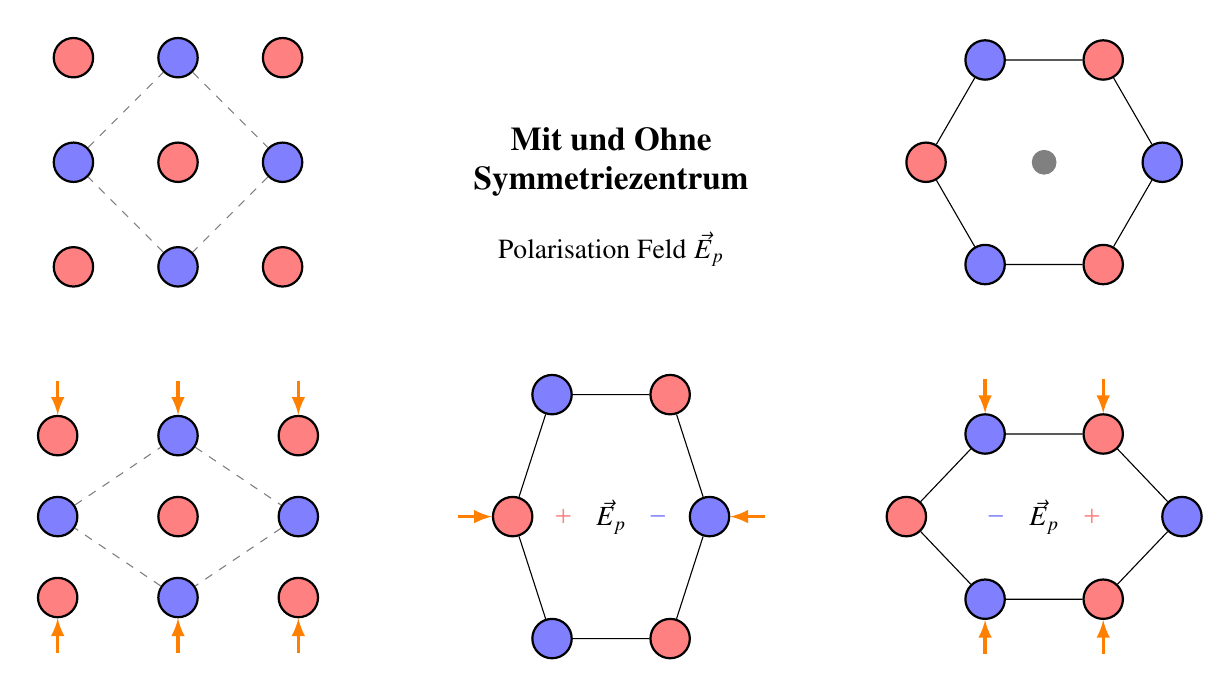
\begin{tikzpicture}[
      >=latex, 
      node distance = 2mm,
      charge/.style = {
        circle, draw = black, thick,
        minimum size = 5mm
      },
      positive/.style = { fill = red!50 },
      negative/.style = { fill = blue!50 },
    ]

    \node[font = {\large\bfseries}, align = center] (title) at (5.5,0) {Mit und Ohne\\ Symmetriezentrum};

    \begin{scope}
      \matrix[nodes = { charge }, row sep = 8mm, column sep = 8mm] {
        \node[positive] {}; & \node[negative] (N) {}; & \node [positive] {}; \\
        \node[negative] (W) {}; & \node[positive] {}; & \node [negative] (E) {}; \\
        \node[positive] {}; & \node[negative] (S) {}; & \node [positive] {}; \\
      };
      \draw[gray, dashed] (W) to (N) to (E) to (S) to (W);
    \end{scope}

    \begin{scope}[xshift=11cm]
      \foreach \x/\t [count=\i] in {60/positive, 120/negative, 180/positive, 240/negative, 300/positive, 360/negative} {
        \node[charge, \t] (C\i) at (\x:1.5cm) {};
      }

      \draw[black] (C1) to (C2) to (C3) to (C4) to (C5) to (C6) to (C1);
      \node[circle, draw=gray, fill=gray, outer sep = 0, inner sep = 0, minimum size = 3mm] {};
      % \draw[gray, dashed] (C2) to (C4) to (C6) to (C2);
    \end{scope}

	%% 
    \node[below = of title] {Polarisation Feld \(\vec{E}_p\)};

	%% hex with vertical pressure
    \begin{scope}[xshift=11cm, yshift=-4.5cm]
      \node[charge, positive, yshift=-2.5mm] (C1) at ( 60:1.5cm) {};
      \node[charge, negative, yshift=-2.5mm] (C2) at (120:1.5cm) {};
      \node[charge, positive, xshift=-2.5mm] (C3) at (180:1.5cm) {};
      \node[charge, negative, yshift= 2.5mm] (C4) at (240:1.5cm) {};
      \node[charge, positive, yshift= 2.5mm] (C5) at (300:1.5cm) {};
      \node[charge, negative, xshift= 2.5mm] (C6) at (360:1.5cm) {};

      \draw[black] (C1) to (C2) to (C3) to (C4) to (C5) to (C6) to (C1);
      % \draw[gray, dashed] (C2) to (C4) to (C6) to (C2);

      \foreach \d in {C1, C2} {
        \draw[orange, very thick, <-] (\d) to ++(0,.7);
      }

      \foreach \d in {C4, C5} {
        \draw[orange, very thick, <-] (\d) to ++(0,-.7);
      }

      \node[black] (E) {\(\vec{E}_p\)};
      \begin{scope}[node distance = .5mm]
        \node[red!50, right = of E] {\(+\)};
        \node[blue!50, left = of E] {\(-\)};
      \end{scope}
      % \draw[gray, thick, dotted] (E) to ++(0,2);
      % \draw[gray, thick, dotted] (E) to ++(0,-2);
    \end{scope}

	%% square with vertical pressure 
    \begin{scope}[yshift=-4.5cm]
      \matrix[nodes = { charge }, row sep = 5mm, column sep = 1cm] {
        \node[positive] (NW) {}; & \node[negative] (N) {}; & \node [positive] (NE) {}; \\
        \node[negative] (W) {}; & \node[positive] {}; & \node [negative] (E) {}; \\
        \node[positive] (SW) {}; & \node[negative] (S) {}; & \node [positive] (SE) {}; \\
      };

      \foreach \d in {NW, N, NE} {
        \draw[orange, very thick, <-] (\d) to ++(0,.7);
      }

      \foreach \d in {SW, S, SE} {
        \draw[orange, very thick, <-] (\d) to ++(0,-.7);
      }

      \draw[gray, dashed] (W) to (N) to (E) to (S) to (W);
    \end{scope}

	%% hex with horizontal pressure
    \begin{scope}[xshift=5.5cm, yshift=-4.5cm]
      \node[charge, positive, yshift= 2.5mm] (C1) at ( 60:1.5cm) {};
      \node[charge, negative, yshift= 2.5mm] (C2) at (120:1.5cm) {};
      \node[charge, positive, xshift= 2.5mm] (C3) at (180:1.5cm) {};
      \node[charge, negative, yshift=-2.5mm] (C4) at (240:1.5cm) {};
      \node[charge, positive, yshift=-2.5mm] (C5) at (300:1.5cm) {};
      \node[charge, negative, xshift=-2.5mm] (C6) at (360:1.5cm) {};

      \draw[black] (C1) to (C2) to (C3) to (C4) to (C5) to (C6) to (C1);
      % \draw[gray, dashed] (C2) to (C4) to (C6) to (C2);

      \draw[orange, very thick, <-] (C6) to ++(.7,0);
      \draw[orange, very thick, <-] (C3) to ++(-.7,0);

      \node[black] (E) {\(\vec{E}_p\)};
      \begin{scope}[node distance = .5mm]
        \node[blue!50, right = of E] {\(-\)};
        \node[red!50, left = of E] {\(+\)};
      \end{scope}
      % \draw[gray, thick, dotted] (E) to ++(0,2);
      % \draw[gray, thick, dotted] (E) to ++(0,-2);
    \end{scope}
  \end{tikzpicture}
\end{document}
